\section{Features of Admin Panel}
\hspace{2cm}Admin Panel monitors the application and provide some statistics to admins that give them an idea about the users’ behaviors, revenue, number of errors and updates, trips count and the number of users joined in each month. Also the admin panel provides some features that help to control and view some of the application data.
It provides the following features:
\begin{itemize}
\item \textbf{Statistics}:
\begin{itemize}
    \item Users’ behavior: Shows the monthly performance of the number of trips made, the number of registered passengers and drivers.
    
    \item Govern distribution: Points to the number of passengers in each govern. This helps to clarify which governs uses the application. This will be much useful when it comes to marketing and regional concentration of application advertisement. Governs with low numbers of users registered will need more effort to make them get to know the application.
    
	\item Monthly Revenue: Shows how much the application earned in each month throughout the year.
	
	\item Info Cards: Views a quick non-detailed information about the application’s total users (drivers and passengers), total revenue, number of errors in server’s run time, number of updates made in application’s back-end side.
\end{itemize}
\item \textbf{Offers}: Provides the capability of pushing new offers to passengers with the help of Google Firebase. Simply we add the offer to the main application remote database and pushes notification to the user’s using Google’s Firebase services. 
\newline
\begin{figure}[htp]%
    \center%
    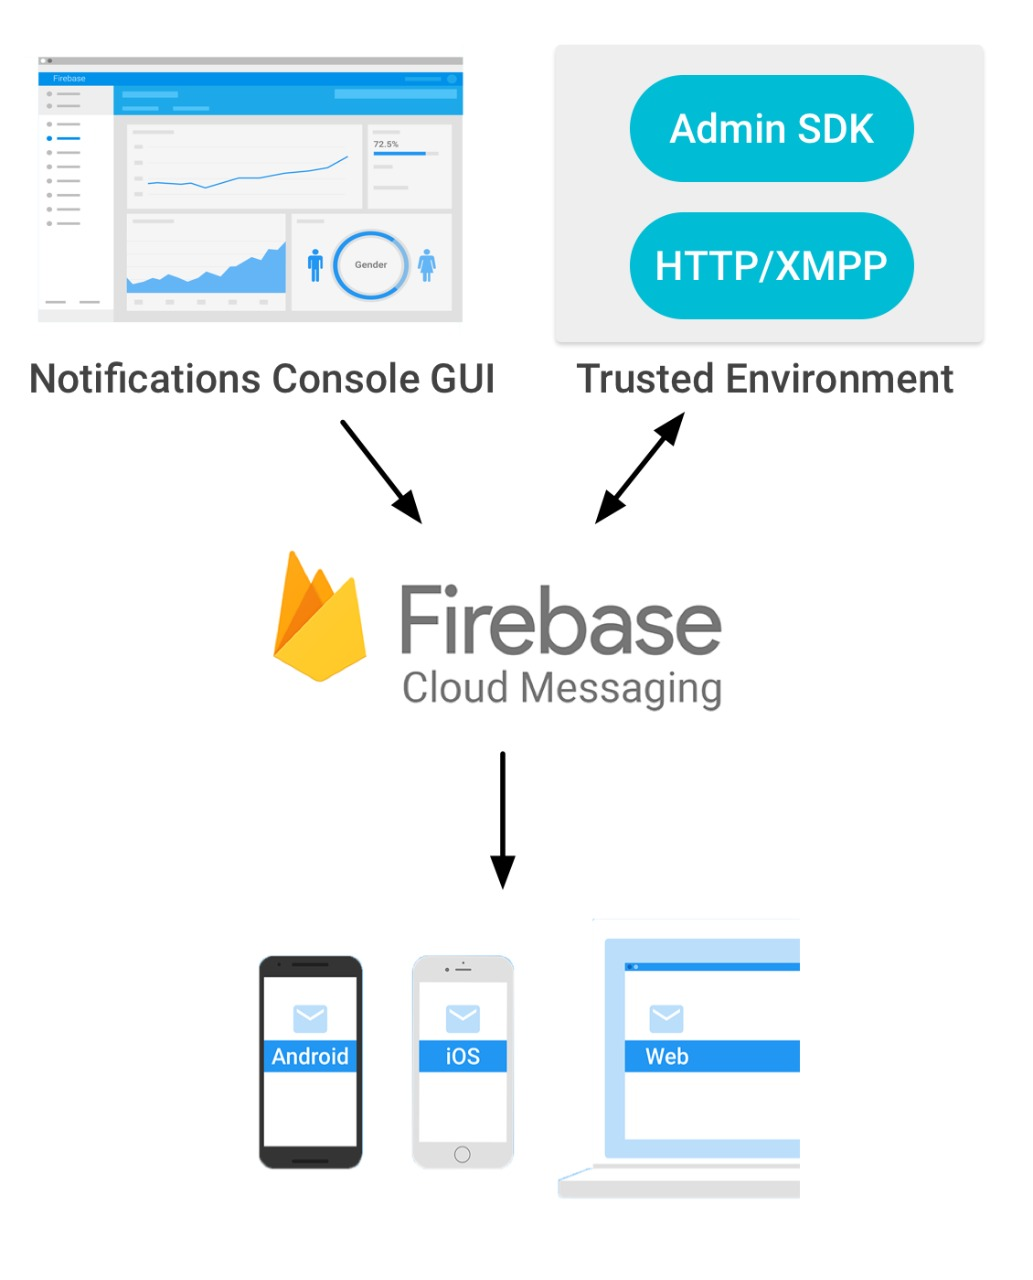
\includegraphics[width=1\textwidth]{images/ch5/fig1.jpg}%
     % you need to add the caption for the list of figures
    \caption[Shows the requests flow between admin panel, firebase and client application.]{Shows the requests flow between admin panel, firebase and client application.}\label{fig: fig1}%
  \end{figure}
  \newline

 These offers can be a discount on any trip the passenger make, a number of totally free trips or a free cash amount added to his wallet. These offers are most likely provided by partners and sponsors to help the application fan base grows. Also it shows the past offers published before and if they are still active or not.
 
\item\textbf{Passengers}: Shows the List of the registered passengers and information about each registered account (name, E-mail, phone, govern, rate, wallet balance, number of trips made and family member) and also gives admins the ability to change some of these data.
Driver Tracking: Admins can live track every active driver using Google maps, to make sure that every driver sticks to his designated route.
\newline
\begin{figure}[htp]%
    \center%
    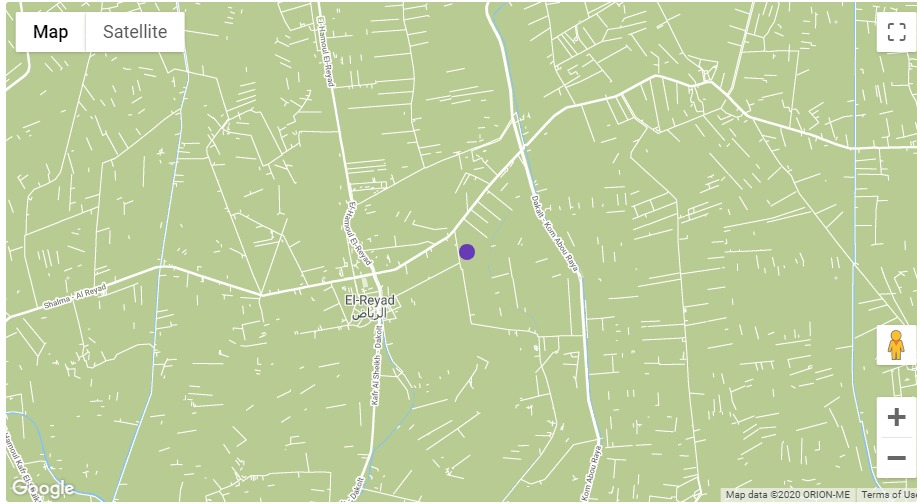
\includegraphics[width=1\textwidth]{images/ch5/fig2.jpg}%
     % you need to add the caption for the list of figures
    \caption[Live location of the selected driver in admin panel.]{Live location of the selected driver in admin panel.}\label{fig:fig2}%
  \end{figure}
  \newline

\item\textbf{Complaints}: Admins can see all users’ complaints and give proper responses to these complaints. 

\item\textbf{Lines}: Views all applications lines and gives the ability to delete or add lines. When adding lines the admin can choose lines’ stations from the map directly and give names to these stations.	
\newline
\begin{figure}[htp]%
    \center%
    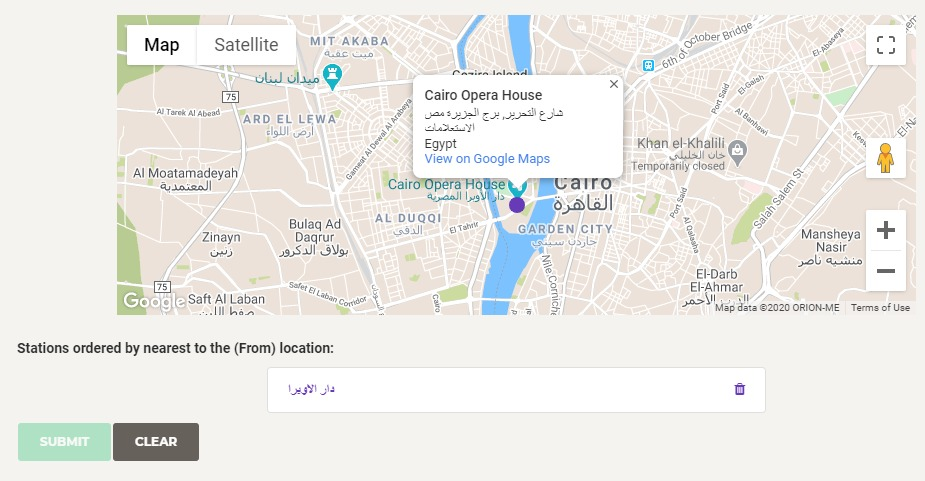
\includegraphics[width=1\textwidth]{images/ch5/fig3.jpg}%
     % you need to add the caption for the list of figures
    \caption[Selecting station location from the map by clicking its location and naming it.]{Selecting station location from the map by clicking its location and naming it.}\label{fig:fig3}%
  \end{figure}
\newline
\item\textbf{Driver Confirmation}: admin can see all drivers sent applications and accept or reject any of which, if they don’t meet the requirements of registration.
\end{itemize}

